% Sample Dissertation, Thesis, or Document %
%            for use with the              %
%  University of Arizona Thesis Class,     %
%               uathesis.cls               %
%------------------------------------------%

% We'll use the uathesis document class (duh).  The uncommented line
% below will produce a Dissertation, the others would produce a Thesis
% or a Document.  There are other options available to you like turning
% on the copyright statement and replacing the year on the title page
% with a "generated on" stamp (handy for early drafts).  To find out
% what the available options are, take a look into the uathesis.cls
% file and look for the \DeclareOption commands near the top of that
% file.
% There are five copyright options.  Copyright, no copyright, and three
% different Creative Commons licences.  Use the one you want (If you go
% Creative Commons, I (DM) think the CC-BY-ND makes the most sense)  See
% uathesis.cls for the reason why the non-commercial licenses are not
% included.
\documentclass[dissertation]{uathesis}
%\documentclass[dissertation,copyright]{uathesis}
%\documentclass[dissertation,CC-BY]{uathesis}
%\documentclass[dissertation,CC-BY-SA]{uathesis}
%\documentclass[dissertation,CC-BY-ND]{uathesis}
%\documentclass[thesis]{uathesis}
%\documentclass[document]{uathesis}

% Package Usage
% These are the packages that we need
\usepackage{graphicx}
\usepackage[square,numbers]{natbib}
\usepackage[titles]{tocloft}
\usepackage{amsmath}
\usepackage{amssymb}
\usepackage{epstopdf}
\usepackage{dcolumn}% Align table columns on decimal point
\usepackage{bm}% bold math
\usepackage{setspace}
\usepackage{rotating}
\renewcommand*\cftfigpresnum{Figure~}
\setlength{\cftfignumwidth}{5.5em}
\renewcommand\cftchapfont{\normalfont}
\renewcommand\cftchappagefont{\normalfont}
\renewcommand\cftchapleader{\cftdotfill{\cftsecdotsep}}

\newcommand\alphaNa{\alpha_\textrm{Na}}
\newcommand\alphaK{\alpha_\textrm{K}}
\newcommand\alphaRb{\alpha_\textrm{Rb}}
\newcommand\alphaCs{\alpha_\textrm{Cs}}
\newcommand\lambdaZero{\lambda_\textrm{zero}}

\newcommand*{\etal}{\emph{et al.}~}

% of the American Astronomical Society.
%\usepackage{deluxetable}		% Allows use of AASTEX deluxe tables
%\usepackage{aastex_hack}		% Allows other AASTEX functionality.

% These are other packages that you might find useful.
% For controlling the fonts, see
% http://www.math.uiuc.edu/~hartke/computer/latex/survey/survey.html
% The following is a nice font set:
%\usepackage{mathtime}			% Times for letters; Belleek math.
%
%\usepackage{lscape}			% Used for making fitting large tables in by putting them landscape
%\usepackage{refs}
%
% If you are using hyper-ref (recommended), this command must go after all
% other package inclusions (from the hyperref package documentation).
% The purpose of hyperref is to make the PDF created extensively
% cross-referenced.
\usepackage[pdftex,bookmarks,colorlinks=true,urlcolor=black,linkcolor=black,citecolor=black]{hyperref}

% Set up some values
\completetitle{Data Driven Solar Power Forecasts}
\fullname{Antonio Tomas Lorenzo}
\degreename{Doctor of Philosophy}	% Title of your degree.

\begin{document}
\newcommand{\beq}{\begin{eqnarray}}
\newcommand{\eeq}{\end{eqnarray}}
\newcommand{\ii}{{\mathrm i}}

% Set up the title page
\maketitlepage
{COLLEGE OF OPTICAL SCIENCES}
{2017}

% Insert the approval form.  Note that for electronic submission
% of your Ph. D. dissertation, you must bring *two* copies of the
% approval page to your final defense.  These must be signed by
% the committee.  Make two photocopies: one for Pam and the other
% for your records.  Then, bring the two signed originals to the
% graduate college when you submit the final version of the
% dissertation to the University of Arizona.
\approval
{14 April 2017}		% Defense Date
{Alexander D. Cronin}	% Dissertation Director
{Matthias Morzfeld}
{Alexander D. Cronin}	% 1st committee member
{Matthias Morzfeld}
{Barrett G. Potter Jr.}


% Include the ``Statement by Author'' for Dissertations
\statementbyauthor
% If this is a Thesis, use the following form, with your thesis director's
% name and title in the square brackets like so (you should also omit the
% approval form insertion above):
%\statementbyauthor[Jane M. Doe\\Professor of Chemistry]

% Include the ``Acknowledgements''
%\incacknowledgements{acknowledgements}

% Include the ``Dedication''
%\incdedication{dedication}

% Create a ``Table of Contents''
\tableofcontents

% Create a ``List of Figures''
\listoffigures

% Create a ``List of Tables''
\listoftables

% Include the ``Abstract''
\incabstract{abstract}

% Include the various chapters
%\chapter{INTRODUCTION}
\label{chap:intro}

The installed capacity of solar power in the US continues to grow as a
result of aging coal and natural gas power plants, lower costs,
state renewable portfolio standards, and efforts to decarbonize the
electrical grid.
As shown in \Cref{fig:solarinstall}, this growth has been steady since 2010 and shows no signs of abating.

\begin{figure}[ht]
  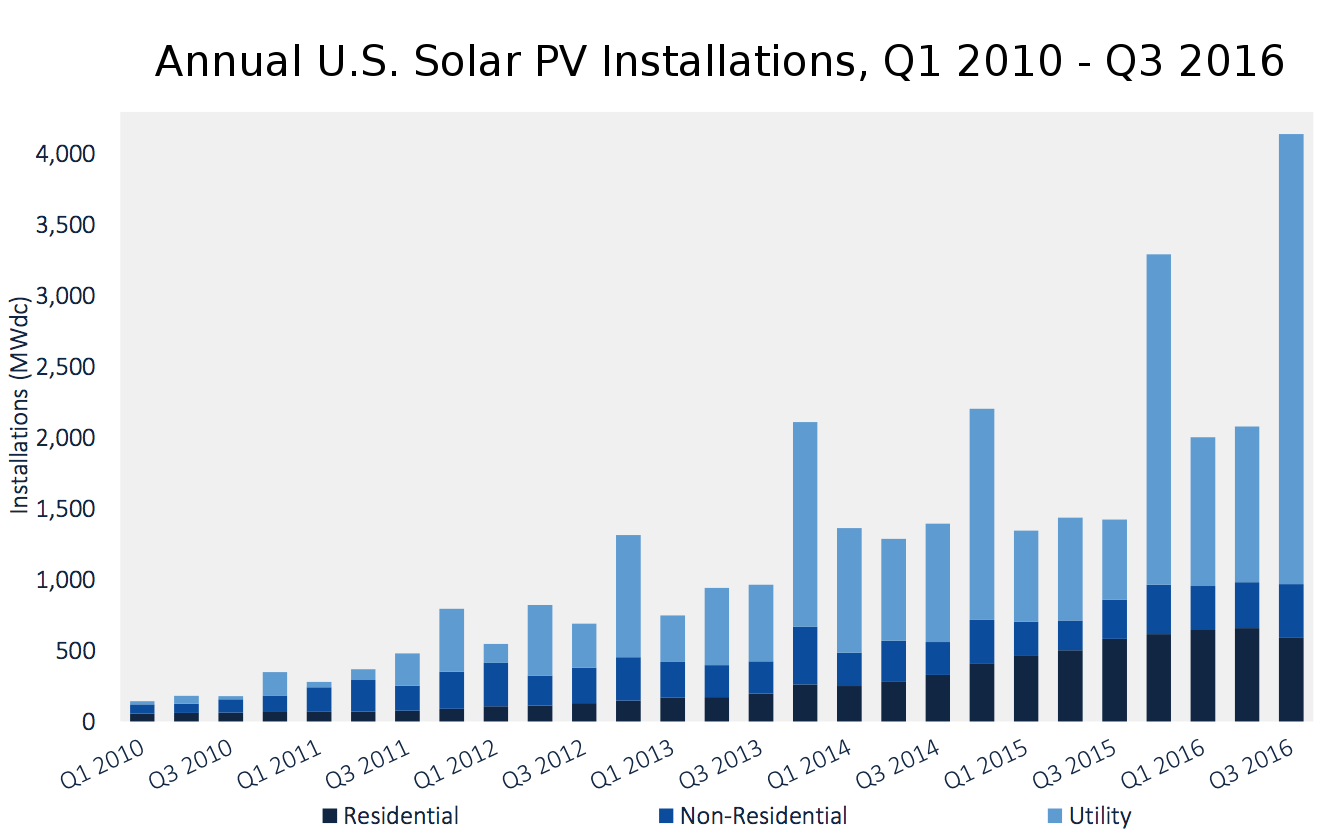
\includegraphics[width=\textwidth]{figs/solar_installations.png}
  \caption[Annual installations of solar PV in the US]{Annual
    installations of solar photovoltaic (PV) systems in the
    US. [Source:~\cite{GTM/SEIA2016}]}
\label{fig:solarinstall}
\end{figure}

Solar irradiance is the fuel that drives all solar power plants.
Unlike sources of fuel for conventional power generators like coal or
natural gas, the solar resource is highly variable due to the nature
of the chaotic system that is weather.
This variability of the solar resource leads to uncertainty at the
electric utility and increases management costs \citep{Joskow2011}.
Forecasts help utilities manage the variability in a number of ways
\citep{Kleissl2013,Inman2013}, including the optimal dispatch of
battery storage \citep{Cormode2015}.

This dissertation will explore solar irradiance forecasting at short
time horizons (now to two hours in the future) made possible by an
irradiance monitoring network.
First, the current state of solar power in the Southwest US and a
brief overview of forecasting methods will be discussed.

\section{State of Solar Power in the Southwest}
duck curve

a bit of SVERI analysis

how much solar total?
percentage of load?

nice heatmap

DG and visibility of DG


\section{Solar Irradiance Forecasting}
nowcasting DG

other techniques

little bit about WRF

\begin{figure}[h]
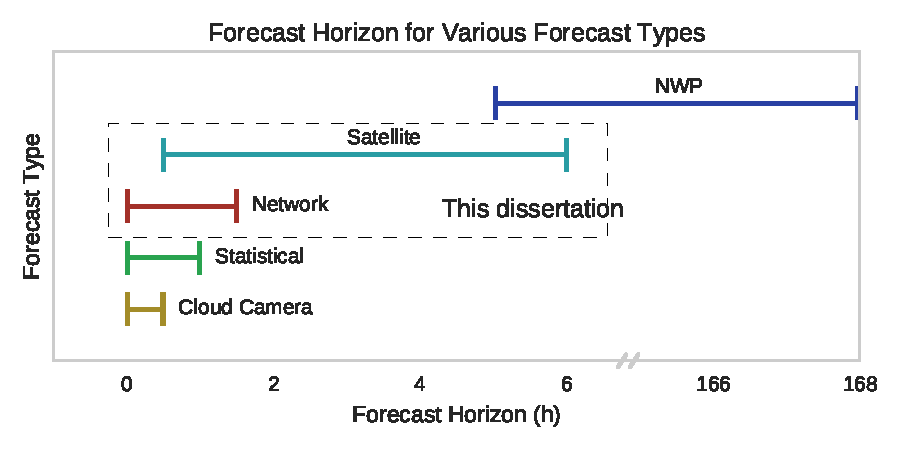
\includegraphics[width=\textwidth]{figs/fxhoriz.pdf}
\caption[Forecast horizon for various forecast types]{The optimal
  forecast horizons for various types of short-term forecasts. This
  dissertation will focus on network and satellite forecasts.}
\label{fig:fxhoriz}
\end{figure}


\section{This Dissertation in Brief}

\begin{figure}[h]
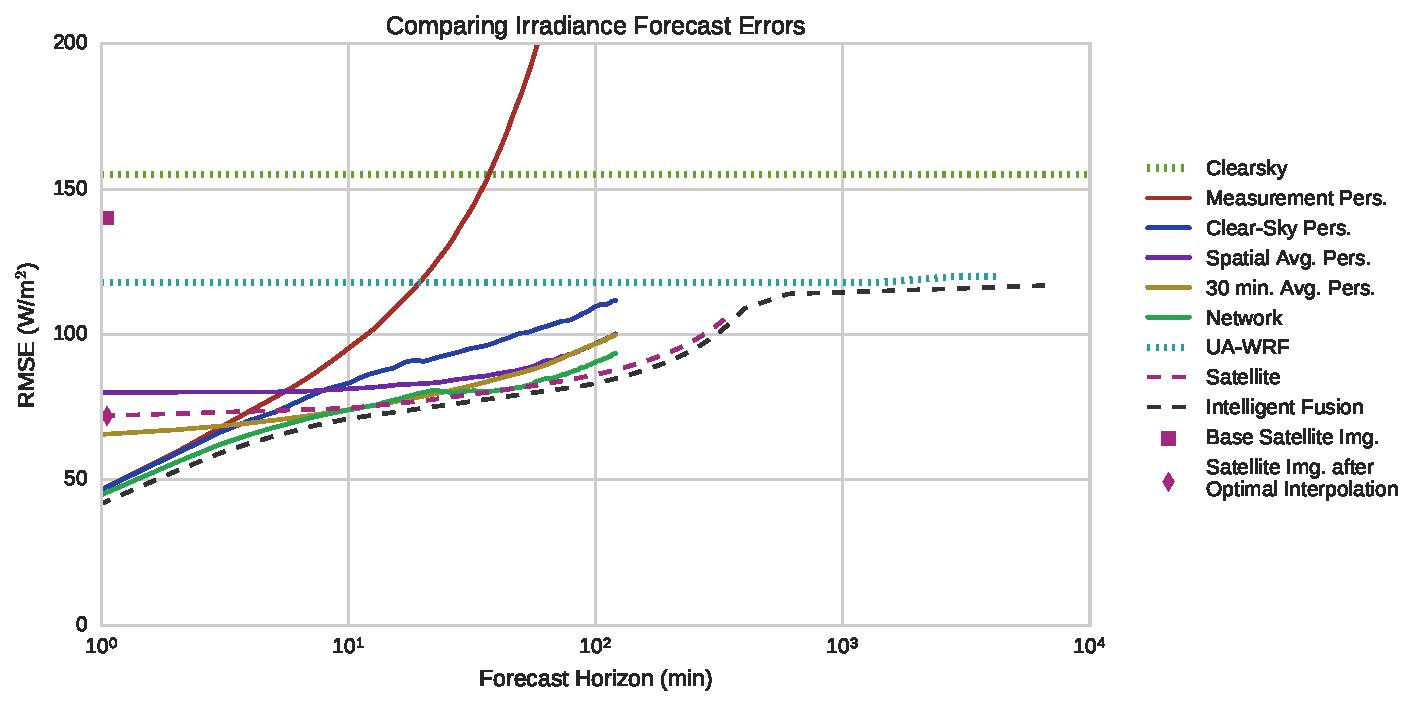
\includegraphics[width=\textwidth]{figs/timehorizon.pdf}
\caption[Irradiance forecast errors across forecast horizons]{A
  comparison of irradiance forecast root-mean squared errors (RMSE)
  across many time horizons. The solid lines (and points) indicate
  forecasts that will be studied in depth in this dissertation. Dashed
  lines are based on prelimnary analysis, but have not been studied in
  depth. Pers.\ refers to persistence, and UA-WRF refers to the
  numerical weather models generated at the UA using the Weather
  Research and Forecasting (WRF) model. The optimal grinding is a
  theoretical combination of forecasts at diffferent time horizons for
  the best forecast at all horizons. The persistence and network
  forecasts will be discussed in \Cref{chap:network} and the satellite
  image points will be discussed in \Cref{chap:satoi}.}
\label{fig:bullshitplot}
\end{figure}




%%% Local Variables:
%%% mode: latex
%%% TeX-master: "dissertation"
%%% End:

%\chapter{CONCLUSION}
\label{chap:conc}

This dissertation has described solar irradiance forecasting
techniques that are used to produce operational solar power forecasts
for utilities.
The techniques rely on data from an irradiance sensor network.
In order to obtain such data, we designed and deployed inexpensive,
remote irradiance sensors throughout Tucson, AZ.
Using data from these sensors, we produced forecasts that improve upon
a reference by reducing RMSE by 20\% for time horizons from one minute
to two hours.
We also carefully analyzed the errors of these forecasts and described
how a smoother forecast may have smaller errors when insufficient care
is taken when analyzing errors.
For longer forecast horizons from 30 minutes to six hours, irradiance
estimates derived from satellite images are used.
Initial satellite estimates had large errors, but we used data
assimilation and data from the sensor network to cut some errors in
half.
Along the way, we studied various methods to estimate the correlation
between pixels in satellite irradiance estimates, including a novel
method based on the difference in cloudiness between two pixels.

Next steps include incorporating a cloud advection model into the data
assimilation routine to produce forecasts and to continuously
incorporate new data while retaining prior information.
These WRF forecasts used for day-ahead and longer forecasts could
benefit from incorporating the actual cloud field at the model
intialization and from an ensemble of model runs.
Eventually, a full physics large eddy simulation of the atmosphere may
be required to properly model the dynamics of clouds and to produce
good forecasts from five minutes to seven days in the future.
We will need to study how to fuse forecasting techniques together
perhaps via machine learning.


%%% Local Variables:
%%% mode: latex
%%% TeX-master: "dissertation"
%%% End:



% Include the various appendices
\appendix
\chapter{REPRINT: IRRADIANCE FORECASTS BASED ON AN IRRADIANCE MONITORING NETWORK, CLOUD MOTION, AND SPATIAL AVERAGING}
\label{app:network}
The following manuscript was published as a peer-reviewed article in
Solar Energy.
Further background material is presented in \Cref{chap:network} of
this dissertation.
The manuscript is reprinted with permission from Elsevier. Original
reference: A. T. Lorenzo, W. F. Holmgren, A. D. Cronin,
2015. Irradiance forecasts based on an irradiance monitoring network,
cloud motion, and spatial averaging. Sol. Energy 122, 1158--1169.
Copyright (2015) by Elsevier.

\newcommand{\figNF}[1]{
\begin{figure}
\includegraphics[ width=1.05\textwidth]{LorenzoSENF/#1}
\end{figure}
}


\figNF{pg1}
\figNF{pg2}
\figNF{pg3}
\figNF{pg4}
\figNF{pg5}
\figNF{pg6}
\figNF{pg7}
\figNF{pg8}
\figNF{pg9}
\figNF{pg10}
\figNF{pg11}
\figNF{pg12}

%%% Local Variables:
%%% mode: latex
%%% TeX-master: "dissertation"
%%% End:

\chapter{LIST OF PUBLICATIONS CO-AUTHORED BY A. T. LORENZO}
Peer-reviewed publications:
\begin{enumerate}

% e.g. \item W.F. Holmgren, R. Trubko, I. Hromada, and A.D. Cronin, \emph{``Measurement of a Wavelength of Light for Which the Energy Shift for an Atom Vanishes"} Physical Review Letters {\bf109}, 243004, (2012).
\item goes here

\end{enumerate}



\noindent Presentations and posters:

\begin{enumerate}

\item poster
%\item Low Energy Seminar, UA Physics Dept., 2010, Talk: \emph{``Absolute and ratio measurements of the polarizability of Na, K, and Rb"} W.F. Holmgren, M.C. Revelle, V.P.A. Lonij, and A.D. Cronin.

%\item Frontiers of Matterwave Optics 2010, Crete, Greece, Poster: \emph{``Absolute and ratio measurements of the polarizability of Na, K, and Rb"} W.F. Holmgren, M.C. Revelle, V.P.A. Lonij, and A.D. Cronin.

\end{enumerate}


\noindent Other works:

\begin{enumerate}

\item other stuff

\end{enumerate}



% Switch the spacing to single-spaced for the references
\renewcommand{\baselinestretch}{1}		% chaning the value
\small\normalsize						% switch size to make the value take

% Create the References list
\bibliographystyle{ieeetran}
\addcontentsline{toc}{chapter}{REFERENCES}
\bibliography{bibliography.bib}

\renewcommand{\baselinestretch}{1.4}		% chaning the value
\small\normalsize						% switch size to make the value take


\end{document}

%%% Local Variables:
%%% mode: latex
%%% TeX-master: t
%%% End:
